\documentclass[10 pt,a 4 paper]{article}
\usepackage[margin=24 mm]{geometry}
\usepackage[T 1]{fontenc}
\usepackage{lmodern,amsmath,amssymb,booktabs,longtable,graphicx,microtype}
\usepackage[numbers,sort&compress]{natbib}
\usepackage[colorlinks=true,allcolors=blue]{hyperref}
\usepackage{xurl}
\graphicspath{{../Figures/}}
\renewcommand{\thesection}{S\arabic{section}}
\renewcommand{\theequation}{S\arabic{equation}}
\renewcommand{\thetable}{S\arabic{table}}
\renewcommand{\thefigure}{S\arabic{figure}}
\title{Supplementary material: Global loss bounds and one-bit recovery for direction-normalized half-moons}
\author{Meshaal Mouawad}
\date{}
\begin{document}
\maketitle
\noindent This supplement supplies complete proofs, numerical certification, experimental details and additional results for the main article. The accompanying reproducibility archive contains machine-readable outputs and the exact implementation. Manuscript displacement $h$ corresponds to the archived generator's gap parameter through $h=-g$.
% Supplementary theory fragment. The wrapper supplies S-prefixed numbering.
% Requires amsmath, amssymb, booktabs and natbib.
\section{Population model and the ray-cancellation identity}
\label{supp:bayes}

Let $a=4/5$, $b=6/5$, $m_0=(0,0)$ and $m_1=(1,h)$, with $h=-g$. Define
\begin{align}
 S_0&=\{x:a<\|x\|<b,\ x_2>0\},\nonumber\\
 S_1&=\{x:a<\|x-m_1\|<b,\ x_2<h\}.
 \label{supp:eq:supports}
\end{align}
Write $H=\pi(b^2-a^2)/2=2\pi/5$ and $K=1/[\pi(b-a)]$. The class densities used in the study are
\begin{equation}
 f_i^A(x)=\frac{\mathbf1_{S_i}(x)}H,
 \qquad
 f_i^R(x)=\frac{K\mathbf1_{S_i}(x)}{\|x-m_i\|}.
 \label{supp:eq:densities}
\end{equation}
The first is uniform with respect to planar area. The second results from independent uniform radius on $(a,b)$ and uniform angle on the appropriate semicircle; the planar area element is $s\,ds\,d\phi$. Boundaries have probability zero. The experiments use $\pi_0=\pi_1=1/2$. Statements involving arbitrary priors assume $\pi_i>0$ and $\pi_0+\pi_1=1$.

For $x\ne c$, the retained representation is $T_c(x)=(x-c)/\|x-c\|$. Its value at $x=c$ can be assigned arbitrarily. Put $u_\theta=(\cos\theta,\sin\theta)$ and
\[
 q_{i,c}(\theta)=\int_0^\infty f_i(c+ru_\theta)r\,dr.
\]
Polar change of variables gives $\int_0^{2\pi}q_{i,c}=1$. The raw and directional Bayes risks are
\begin{align}
 R_X^*&=\int_{\mathbb R^2}\min\{\pi_0f_0(x),\pi_1f_1(x)\}\,dx,
 \label{supp:eq:raw-risk}\\
 R^*_{T_c}&=\int_0^{2\pi}\min\{\pi_0q_{0,c}(\theta),
                                  \pi_1q_{1,c}(\theta)\}\,d\theta.
 \label{supp:eq:direction-risk}
\end{align}
Let $d=\pi_0f_0-\pi_1f_1$ and define
\[
 A_c(\theta)=\int_0^\infty[d(c+ru_\theta)]_+r\,dr,
 \qquad
 B_c(\theta)=\int_0^\infty[-d(c+ru_\theta)]_+r\,dr.
\]
Since $\min(s,t)=(s+t-|s-t|)/2$,
\begin{align*}
 R_X^*&=\frac12\left(1-\int_0^{2\pi}(A_c+B_c)\,d\theta\right),\\
 R^*_{T_c}&=\frac12\left(1-\int_0^{2\pi}|A_c-B_c|\,d\theta\right).
\end{align*}
Subtracting proves
\begin{equation}
 \Delta(c):=R^*_{T_c}-R_X^*
 =\int_0^{2\pi}\min\{A_c(\theta),B_c(\theta)\}\,d\theta.
 \label{supp:eq:cancellation}
\end{equation}
In particular, zero loss holds exactly when almost every ray carries at most one strict sign of $d$. This is the binary zero--one specialization of representation-induced Bayes loss \citep{Silva2012,Silva2024}.

\section{Connected winner regions and the disjoint-support transition}
\label{supp:geometry}

For a set $U$, write
\[
 \Omega_c(U)=\{(x-c)/\|x-c\|:x\in U\setminus\{c\}\}
\]
for its angular image. If $U$ is open and $c\in U$, then $\Omega_c(U)$ is the full circle. If $U$ is connected and $c\notin U$, continuity and openness of the direction map show that $\Omega_c(U)$ is a connected open subset of the circle: an open arc or the full circle.

\paragraph{Lemma 1 (mutual convex-hull intrusion).}
Suppose connected open sets $U_0,U_1$ satisfy $d>0$ almost everywhere on $U_0$, $d<0$ almost everywhere on $U_1$, and
\begin{equation}
 U_0\cap\operatorname{int}\operatorname{conv}(U_1)\ne\varnothing,
 \qquad
 U_1\cap\operatorname{int}\operatorname{conv}(U_0)\ne\varnothing.
 \label{supp:eq:intrusion}
\end{equation}
Then $\Delta(c)>0$ for every $c\in\mathbb R^2$. This criterion is a probabilistic adaptation of the separability geometry developed by Hurtado et al.\ \citep{Hurtado2001}.

\emph{Proof.}
If the angular images overlap, their intersection is open. Every ray in this intersection meets each $U_i$ in a nonempty open radial interval. Polar Fubini and the almost-everywhere strict signs imply $A_c,B_c>0$ for almost every angle in that intersection. Equation~\eqref{supp:eq:cancellation} then gives positive loss.

Suppose instead that the images are disjoint. Neither can be the full circle, so they are disjoint open arcs. At least one, say $\Omega_c(U_0)$, has length at most $\pi$. The set
\[
 C=\{ru:r>0,\ u\in\Omega_c(U_0)\}
\]
is convex: positive sums of vectors whose directions belong to an open arc of length at most $\pi$ retain a direction in that arc and cannot equal zero. Consequently $\operatorname{conv}(U_0)-c\subseteq C$. A point of $U_1\cap\operatorname{conv}(U_0)$ therefore has a direction in both angular images, contradicting disjointness. This proves the lemma.\hfill$\square$

\paragraph{Proposition 1 (the disjoint nonlinear interval).}
For $0<h\leq\sqrt{3/5}$, $S_0\cap S_1=\varnothing$. For any positive priors and class densities positive almost everywhere on these supports,
\begin{equation}
 R_X^*=0,\qquad\Delta(c)>0\quad(c\in\mathbb R^2).
 \label{supp:eq:disjoint-result}
\end{equation}
For $h\leq0$, every origin satisfying $h\leq c_2\leq0$ has zero directional risk.

\emph{Proof.}
Assume first $0<h\leq\sqrt{3/5}<a$. A common point must have height $0<y<h$. Set
\[
 s(y)=\sqrt{a^2-y^2},\qquad t(y)=\sqrt{b^2-y^2}.
\]
The horizontal intervals of the two supports at that height are
\begin{align*}
 S_0:&\quad(-t(y),-s(y)),\quad(s(y),t(y)),\\
 S_1:&\quad(1-t(h-y),1-s(h-y)),\quad
                  (1+s(h-y),1+t(h-y)).
\end{align*}
The derivative
\[
 \frac{d}{dy}\{t(h-y)-s(y)\}
 =\frac{h-y}{t(h-y)}+\frac y{s(y)}\geq0
\]
gives $t(h-y)-s(y)\leq b-s(h)$. Interchanging $y$ and $h-y$ gives the corresponding reversed bound. Concavity of $s$ gives
\[
 s(y)+s(h-y)\geq a+s(h).
\]
When $s(h)\geq1/5$, these inequalities separate the left intervals of the two classes, the right intervals, and the potentially crossing middle pair. The remaining pair is already ordered by sign. Thus all pairs are disjoint. The condition $s(h)\geq1/5$ is equivalent to $h\leq\sqrt{3/5}$; equality permits boundary contacts only. For $\sqrt{3/5}<h<a$, the class-0 right interval and class-1 left interval overlap at heights sufficiently close to zero, establishing the threshold within $0\leq h<a$.

Each support is connected and open. Its convex hull is the open outer half-disk with the same center and orientation. The point $z_0=(1,h/2)$ has class-0 radius $\sqrt{1+h^2/4}\in(a,b)$ and lies strictly inside the class-1 outer half-disk. Its reflection $z_1=(0,h/2)$ gives the reverse intrusion. Because disjoint supports have opposite signs of $d$, Lemma~1 proves positive directional risk for every origin. Raw risk is zero by disjointness.

For $h\leq0$ and $h\leq c_2\leq0$, every class-0 observation has positive vertical direction and every class-1 observation has negative vertical direction. The direction therefore determines the class almost surely.\hfill$\square$

\section{An exclusive-region construction for overlapping supports}
\label{supp:overlap}

Set $h=1$. The point $(9/10,1/10)$ lies strictly inside both supports: its squared distances to the two centers are both $82/100$, between $a^2$ and $b^2$. A neighborhood of that point belongs to the overlap. Positive almost-everywhere class densities and positive priors therefore give $R_X^*>0$.

To establish strictly positive additional loss at every origin, define
\begin{align*}
 w_1&=(1,1/4),&w_2&=(-1,1/20),&w_3&=(0,11/10),\\
 v_i&=(1,1)-w_i.&&&
\end{align*}
Let $R=11/10$, $\theta_0=\arctan(1/4)$ and
$\theta_1=\pi-\arctan(1/20)$. Form a compact connected set $K_0$ from the circular arc
\[
 \{R(\cos\theta,\sin\theta):\theta_0\leq\theta\leq\theta_1\}
\]
and the radial segments joining $w_1,w_2$ to the two arc endpoints. The arc contains $w_3$. Put $K_1=(1,1)-K_0$ and $\rho=1/20$.

Every open radius-$\rho$ disk centered on $K_0$ is contained in $S_0\setminus\overline{S_1}$. To verify its class-0 inclusion, every center has radius between $\sqrt{401}/20>1$ and $11/10$, and height at least $1/20$. The disk therefore stays strictly between the class-0 radial boundaries and above its diameter. Exclusion from class 1 follows by checking the pieces of $K_0$:

\begin{enumerate}
\item On the radial segment from $w_1$, write $x=\lambda(1,1/4)$, where $1\leq\lambda\leq22/(5\sqrt{17})$. The squared distance to $(1,1)$ is $17\lambda^2/16-5\lambda/2+2$ and decreases on that interval. Its maximum is $9/16$. A radius-$1/20$ disk is therefore contained in the opposite inner hole of radius $4/5$.
\item On the radial segment from $w_2$, the first coordinate is at most $-1$, so the distance to $(1,1)$ is at least $2>b+\rho$.
\item On the right circular branch up to height $21/20$, the squared distance to $(1,1)$ is
\[
 321/100-2R(\cos\theta+\sin\theta)
 \leq321/100-11/\sqrt{17}<9/16.
\]
The minimum of $\cos\theta+\sin\theta$ on this arc segment occurs at an endpoint. The starting endpoint gives $x_1+x_2=11/(2\sqrt{17})$; the other gives $(21+\sqrt{43})/20$, which is larger. These disks are again inside the class-1 inner hole.
\item On the central arc with height at least $21/20$, the entire open disk lies above the class-1 diameter $x_2=1$.
\item On the remaining left branch below height $21/20$, $x_1\leq-\sqrt{43}/20$. Hence the distance to $(1,1)$ is at least $1+\sqrt{43}/20>5/4=b+\rho$.
\end{enumerate}
Reflection gives the same exclusive-region clearance for $K_1$. Thus
\[
 U_i=K_i+B(0,\rho)
\]
are connected open subsets of the corresponding exclusive regions, where $B$ denotes an open disk. The exact identity
\begin{equation}
 v_1=\frac7{38}w_1+\frac7{38}w_2+\frac{12}{19}w_3
 \label{supp:eq:barycentric}
\end{equation}
has strictly positive coefficients. Since the three $w_i$ are noncollinear, $v_1$ lies in the interior of their triangle, which is contained in $\operatorname{conv}(U_0)$. Reflection gives the reverse intrusion. The signs of $d$ are fixed and opposite on the exclusive sets for every pair of positive priors. Lemma~1 proves
\begin{equation}
 R^*_{T_c}>R_X^*>0\qquad(c\in\mathbb R^2, h=1).
 \label{supp:eq:overlap-result}
\end{equation}

\section{Exterior certificates and a positive global infimum}
\label{supp:exterior}

\paragraph{A general disk construction.}
Let $K_0,K_1$ be compact connected sets. Suppose each open radius-$\rho$ disk centered on $K_0$ lies where $d\geq\kappa_0>0$ almost everywhere, and each such disk centered on $K_1$ lies where $d\leq-\kappa_1<0$ almost everywhere. Suppose also that
\[
 B(p,\delta)\subseteq\operatorname{conv}(K_0)\cap\operatorname{conv}(K_1),
 \qquad \|x-p\|\leq M\quad(x\in K_0\cup K_1).
\]
Then, for $t=\|c-p\|>M+\rho$,
\begin{equation}
 \Delta(c)\geq4\rho(t-M)\arcsin(\delta/t)
                   \min(\kappa_0,\kappa_1).
 \label{supp:eq:general-exterior}
\end{equation}

To prove this, observe first that a compact connected set viewed from outside its convex hull has the same angular image as its convex hull. Strict separation from the origin places the angular image in an interval shorter than a semicircle. Connectedness fills the interval between the extreme directions, and convex combinations introduce no additional extreme direction. Since $t>M$, the observation applies to each $K_i$. Every ray crossing $B(p,\delta)$ therefore meets both $K_i$. A meeting point is at radial distance $r_i\geq t-M>\rho$ from $c$. Its radius-$\rho$ disk contributes signed ray mass at least
\[
 \kappa_i\int_{r_i-\rho}^{r_i+\rho}r\,dr
 =2\kappa_i\rho r_i\geq2\kappa_i\rho(t-M).
\]
The common disk subtends an angle $2\arcsin(\delta/t)$. Applying~\eqref{supp:eq:cancellation} proves~\eqref{supp:eq:general-exterior}. If $M>\rho$ and $t\geq2M$, the inequalities $\arcsin z\geq z$ and $(t-M)/t\geq1/2$ give
\begin{equation}
 \Delta(c)\geq2\rho\delta\min(\kappa_0,\kappa_1).
 \label{supp:eq:constant-exterior}
\end{equation}

\paragraph{The disjoint geometry $h=1/2$.}
Use
\[
 \rho=\delta=\frac18,\qquad p=(1/2,1/4),\qquad
 M=\frac{43}{40}+\frac{\sqrt5}{4},
\]
and the eroded supports
\[
 E_0=\{x:a+\rho\leq\|x\|\leq b-\rho,\ x_2\geq\rho\},
 \qquad E_1=(1,1/2)-E_0.
\]
These are compact connected annular caps, and every open radius-$\rho$ disk centered on $E_i$ lies in $S_i$. Their convex hulls are the outer disk caps
\[
 \operatorname{conv}(E_0)=\{x:\|x\|\leq b-\rho,\ x_2\geq\rho\},
 \qquad\operatorname{conv}(E_1)=(1,1/2)-\operatorname{conv}(E_0).
\]
Indeed, the entire outer circular arc belongs to $E_0$, and its convex hull is the displayed cap. The common disk $B(p,\delta)$ lies in both hulls: its heights lie between $1/8$ and $3/8$, and $\|p\|+\delta<b-\rho$. Each point of either eroded support satisfies $\|x-p\|\leq b-\rho+\|p\|=M$. Hence~\eqref{supp:eq:general-exterior} applies with $K_i=E_i$ and
\[
 \kappa_i=\frac{\pi_i}{H}\quad\hbox{for area},
 \qquad
 \kappa_i=\pi_i\frac{K}{b}=\pi_i\frac{25}{12\pi}
 \quad\hbox{for radius}.
\]
Here each support is exclusive because $h=1/2$ is in the disjoint interval. In particular, for equal priors and $\|c-p\|\geq2M=43/20+\sqrt5/2$,
\begin{equation}
 \Delta_A(c)\geq\frac5{128\pi},\qquad
 \Delta_R(c)\geq\frac{25}{768\pi}.
 \label{supp:eq:disjoint-exterior}
\end{equation}

\paragraph{The overlapping geometry $h=1$.}
Use the exclusive backbones of Section~\ref{supp:overlap}, with
\[
 \rho=\frac1{20},\qquad\delta=\frac18,
 \qquad p=(1/2,1/2),\qquad M=\frac{11}{10}+\frac1{\sqrt2}.
\]
The point $p$ has barycentric weights $(45,7,24)/76$ in the triangle $w_1w_2w_3$. Its distances to the three edge lines are
\[
 \frac3{\sqrt{101}},\qquad\frac7{2\sqrt{689}},\qquad\frac{45}{58},
\]
all larger than $1/8$. Thus the triangle contains $B(p,\delta)$. Reflection about $p$ establishes its inclusion in both backbone convex hulls. Moreover, $\|x-p\|\leq11/10+\|p\|=M$ on either backbone. Their exclusive-region clearance supplies the same $\kappa_i$ as above. For equal priors and $\|c-p\|\geq2M=11/5+\sqrt2$,
\begin{equation}
 \Delta_A(c)\geq\frac1{64\pi},\qquad
 \Delta_R(c)\geq\frac5{384\pi}.
 \label{supp:eq:overlap-exterior}
\end{equation}

\paragraph{Relation to the global bounds.}
The displayed constants certify exterior origins. The general projection-limit theorem in Section~\ref{supp:projection-boundary} establishes positive global loss for arbitrary positive-a.e. densities throughout the disjoint interval and at $h=1$. Section~\ref{supp:constructive-global} converts the cores above into explicit lower certificates over the entire origin plane.

\section{A finite necessary and sufficient preservation test}
\label{supp:finite}

For a fixed origin $c$, use the four circles with centers $m_0,m_1$ and radii $a,b$, and the diameter lines $x_2=0,h$. Full circles and lines can be used: their unused portions only refine the partition. Collect these oriented direction events:
\begin{enumerate}
\item Tangent directions from $c$ to every circle, including both limiting tangent directions when $c$ lies on the circle.
\item Directions from $c$ to every pairwise curve intersection other than $c$ itself.
\item The four coordinate directions, which include the diameter-line parallel directions and ensure that every angular cell has length less than $\pi$.
\end{enumerate}
Merge repeated directions and coincident curves. The six circle pairs have at most $12$ intersections; the eight circle--line pairs have at most $16$. The diameter lines are parallel or coincident. Adding at most eight tangencies and four coordinate directions gives at most $40$ distinct events.

Select one interior direction in each nonempty angular cell. Order all positive intersection radii on its ray, include the endpoint $r=0$, and inspect one point of each intervening open radial interval. For area densities, support membership determines the sign of $d$: positive on class-0-exclusive intervals, negative on class-1-exclusive intervals, and the sign of $\pi_0-\pi_1$ on overlap intervals. Intervals outside both supports have zero sign. The decision is
\begin{equation}
 \Delta(c)>0
 \quad\Longleftrightarrow\quad
 \text{at least one tested ray contains intervals of both strict signs.}
 \label{supp:eq:finite-test}
\end{equation}

\emph{Completeness proof.}
Within an open angular cell, simple positive roots vary continuously. Circle roots can be created or destroyed only at a tangent direction, and line roots can escape to infinity only at a parallel direction. The order of distinct positive roots can change only when a ray meets an intersection of two curves. These are all recorded events. Therefore each radial interval retains its support-membership pattern throughout the cell. Both strict signs at the test direction imply both signs on the entire cell; polar Fubini and~\eqref{supp:eq:cancellation} give positive loss. Conversely, if every cell has at most one strict sign, almost every angle has zero cancellation. The finite set of event directions has zero angular measure, proving zero loss.

For radius densities, the sign within an overlap interval is determined by
\begin{equation}
 P(x)=\pi_0^2\|x-m_1\|^2-\pi_1^2\|x-m_0\|^2.
 \label{supp:eq:apollonius}
\end{equation}
Both distances are strictly positive on the supports, so squaring the comparison $\pi_0/\|x-m_0\|$ versus $\pi_1/\|x-m_1\|$ preserves its sign. Include $P(x)=0$ in the arrangement. For equal priors this curve is the line
\[
 x_1+hx_2=(1+h^2)/2.
\]
It contributes at most eight circle intersections, two diameter-line intersections and two parallel directions, giving at most $52$ events. Unequal positive priors produce an Apollonius circle. Its at most eight circle intersections, four line intersections and two tangencies give at most $54$ events. The refined radial intervals now have constant signed-density sign, so the same proof establishes~\eqref{supp:eq:finite-test}.

\paragraph{Degenerate events and exact arithmetic.}
If $c$ lies on a circle, its zero root persists for all directions; the other root crosses zero at the two tangent directions, which are included. If $c$ lies on a line, the zero root again persists; rays lying on that line are its two parallel event directions. An intersection point equal to $c$ contributes no defined direction and is omitted, with its changes already handled by these tangent or parallel events. Coincident curves are represented once, roots sharing a radius are merged, and zero-length radial intervals are discarded. Tangencies between different curves produce a single intersection event. Equal priors in the area model give zero signed density throughout an overlap interval, so ties are assigned sign zero. The unbounded last radial interval has zero density because the supports are bounded.

For rational $a,b,h,c$ and priors, circle intersections, tangent directions and ray roots are algebraic. Coordinate events ensure adjacent directions differ by less than $\pi$, so their normalized vector sum gives an algebraic interior test direction. Algebraic root ordering and sign evaluation implement the finite decision exactly.

\paragraph{A quantitative witness from one cell.}
Suppose a test ray contains points $x_\pm=c+r_\pm u_{\theta_0}$ in opposite winning regions. Choose $0<\epsilon_\pm<r_\pm$ and $\kappa_\pm>0$ so that $d\geq\kappa_+$ on $B(x_+,\epsilon_+)$ and $d\leq-\kappa_-$ on $B(x_-,\epsilon_-)$ almost everywhere. Put
\[
 \alpha=\min\{\epsilon_+/(2r_+),\epsilon_-/(2r_-)\}.
\]
For $|\theta-\theta_0|\leq\alpha$ and $|r-r_i|\leq\epsilon_i/2$,
\[
 \|ru_\theta-r_i u_{\theta_0}\|
 \leq|r-r_i|+r_i\|u_\theta-u_{\theta_0}\|\leq\epsilon_i.
\]
The corresponding signed ray mass is at least $\kappa_i r_i\epsilon_i$, giving
\begin{equation}
 \Delta(c)\geq2\alpha\min\{\kappa_+r_+\epsilon_+,
                              \kappa_-r_-\epsilon_-\}>0.
 \label{supp:eq:witness}
\end{equation}
Area-model margins are constant on each winning interval. Radius-model margins have a positive lower bound on any sufficiently small closed disk away from the support boundaries and decision curve.

\section{Exact radial and horizontal integrals}
\label{supp:radial}

For class $i$, put $v=c-m_i$, $z=u_\theta^Tv$ and $D^2=\|v\|^2$. Intersections of the ray with a circle of radius $R$ satisfy
\[
 r^2+2zr+D^2-R^2=0,
 \qquad r=-z\pm\sqrt{z^2+R^2-D^2}.
\]
Negative discriminants give no intersection; a zero discriminant is a tangency. Keep the positive interval inside the outer disk, remove the interval inside the inner disk, and intersect with the appropriate half-plane condition
\[
 \sigma_i(v_2+r\sin\theta)>0,
 \qquad\sigma_0=1,\quad\sigma_1=-1.
\]
If $\sin\theta=0$, this condition either retains or removes the whole interval according to the sign of $\sigma_i v_2$. A ray lying on the diameter is an exceptional boundary direction. This construction leaves at most two nonempty intervals $[\ell,u]$ for a class; endpoints do not affect their integrals.

For area sampling, such an interval contributes
\begin{equation}
 \int_\ell^u f_i^A(c+ru_\theta)r\,dr
 =\frac{u^2-\ell^2}{2H}.
 \label{supp:eq:area-primitive}
\end{equation}
For radius sampling, let $k^2=D^2-z^2$. If $k>0$, define
\begin{equation}
 F(r)=\sqrt{(r+z)^2+k^2}
       -z\operatorname{arsinh}((r+z)/k).
 \label{supp:eq:radius-primitive}
\end{equation}
Differentiation gives
\[
 F'(r)=\frac{r+z}{\sqrt{(r+z)^2+k^2}}
        -\frac z{\sqrt{(r+z)^2+k^2}}
       =\frac r{\|v+ru_\theta\|}.
\]
The interval contribution is therefore $K[F(u)-F(\ell)]$. In the collinear case $k=0$, use
\begin{equation}
 F(r)=|r+z|-z\operatorname{sign}(r+z)\log|r+z|
 \label{supp:eq:collinear-primitive}
\end{equation}
on each side of $r+z=0$. The annulus has inner radius $a>0$, so a retained interval cannot meet this singular point. At the class-centered origin $c=m_i$, $z=k=0$ and $F(r)=r$ for $r>0$. Summing interval contributions gives $q_{i,c}$, and~\eqref{supp:eq:direction-risk} leaves one angular integration.

\paragraph{Area raw risk.}
The constant class densities give
\begin{equation}
 R_{X,A}^*=\frac{\min(\pi_0,\pi_1)}H\,|S_0\cap S_1|.
 \label{supp:eq:raw-area}
\end{equation}
At a height $y$, the circle roots are $m_{i1}\pm\sqrt{R^2-(y-m_{i2})^2}$. Split the height axis at diameter levels, circle extrema and heights of circle intersections. Between consecutive events their order is fixed, so the overlap length is a sum of constants and signed square roots. The primitive
\begin{equation}
 G_R(s)=\frac{s\sqrt{R^2-s^2}+R^2\arcsin(s/R)}2
 \label{supp:eq:circle-area-primitive}
\end{equation}
integrates each root term. This gives an elementary finite evaluation of~\eqref{supp:eq:raw-area}.

\paragraph{Radius raw risk.}
For a direct horizontal calculation, partition each horizontal overlap interval additionally at roots of~\eqref{supp:eq:apollonius}. On each resulting interval choose the smaller weighted density. Its primitive for class $i$ is
\begin{equation}
 K\operatorname{arsinh}\!\left(\frac{x_1-m_{i1}}{|y-m_{i2}|}\right),
 \qquad y\ne m_{i2}.
 \label{supp:eq:horizontal-radius}
\end{equation}
At $y=m_{i2}$, the corresponding primitive on either side of the excluded class center is $K\operatorname{sign}(x_1-m_{i1})\log|x_1-m_{i1}|$. Multiply by $\pi_i$, sum the retained differences, and integrate over height.

At equal priors there is also a symmetric polar form. Reflection $x\mapsto m_1-x$ swaps the class densities and the two halves of their overlap separated by the perpendicular bisector. The lower density is the density from the more distant center, so
\begin{equation}
 R_{X,R}^*
 =\mathbb P_0^R\{X\in S_1,\ \|X\|\geq\|X-m_1\|\}.
 \label{supp:eq:raw-radius-symmetry}
\end{equation}
In polar coordinates $X=ru_\theta$ about $m_0$, the last condition becomes
$r(u_\theta^Tm_1)\geq\|m_1\|^2/2$. The density times the area element is $K\,dr\,d\theta$, so the raw risk equals $K$ times the angular integral of the radial lengths satisfying this condition and both support constraints.

\section{Comparison of the two sampling laws}
\label{supp:density}

On each class support,
\begin{equation}
 \frac{f_i^R(x)}{f_i^A(x)}
 =\frac{a+b}{2\|x-m_i\|}\in[\alpha,\beta],
 \qquad\alpha=\frac56,\quad\beta=\frac54.
 \label{supp:eq:density-ratio}
\end{equation}
Integration and monotonicity of the minimum imply
\[
 \alpha R_{X,A}^*\leq R_{X,R}^*\leq\beta R_{X,A}^*,
 \qquad
 \alpha R_{T_c,A}^*\leq R_{T_c,R}^*\leq\beta R_{T_c,A}^*.
\]
When the supports are disjoint, raw risks vanish, so the same two-sided comparison holds for representation loss. Moreover, all densities positive almost everywhere on those supports have the same zero-loss origin set: an open intersection of angular support images yields positive error, and disjoint images yield zero error.

For equal priors, $d_A=(\mathbf1_{S_0}-\mathbf1_{S_1})/(2H)$ is zero on the overlap. On exclusive regions $d_R$ has the same sign and magnitude at least $\alpha|d_A|$. Hence $[\pm d_R]_+\geq\alpha[\pm d_A]_+$ pointwise. Integrating along rays and using~\eqref{supp:eq:cancellation} gives
\begin{equation}
 \Delta_R(c)\geq\frac56\Delta_A(c)
 \label{supp:eq:density-loss-lower}
\end{equation}
for all origins, including the overlapping geometry. A corresponding upper bound is
\begin{equation}
 \Delta_R(c)\leq\frac54\Delta_A(c)
      +\int_{S_0\cap S_1}|d_R(x)|\,dx.
 \label{supp:eq:density-loss-upper}
\end{equation}
Indeed, on each ray the positive and negative exclusive masses are at most $\beta$ times their area counterparts. Adding the overlap masses can increase their minimum by at most their sum. Polar integration gives~\eqref{supp:eq:density-loss-upper}. Within the overlap, the radius model favors class 0 precisely when $x_1+hx_2<(1+h^2)/2$.

\section{Bounded variation and certified quadrature}
\label{supp:bv}

\paragraph{Angular pushforward bound.}
Let $f$ be a compactly supported planar function of bounded variation, with distributional gradient measure $Df$. Define $J(x_1,x_2)=(-x_2,x_1)$ and $V_c(x)=J(x-c)$. For a smooth periodic function $\varphi$, polar coordinates and integration by parts give
\begin{align*}
 \int_0^{2\pi}q_c(\theta)\varphi'(\theta)\,d\theta
 &=\int_{\mathbb R^2} f(x)V_c(x)\cdot
                    \nabla[\varphi(T_c(x))]\,dx\\
 &=-\int_{\mathbb R^2}\varphi(T_c(x))V_c(x)\cdot Df(x).
\end{align*}
Here $\varphi(T_c(x))$ means the periodic angular function evaluated at the direction. A radial cutoff around $c$ removes its coordinate singularity; $V_c$ is tangent to the cutoff circles, so it contributes no radial boundary flux. The identity first holds for smooth functions, and BV approximation gives the distributional statement. Consequently $D_\theta q_c$ is the angular pushforward of the signed measure $V_c\cdot Df$, and total variation contracts under pushforward:
\begin{equation}
 \operatorname{TV}(q_c)\leq
 |V_c\cdot Df|(\mathbb R^2).
 \label{supp:eq:angular-bv}
\end{equation}

\paragraph{Area density.}
For a half-annulus centered at $m=(m_x,m_y)$, write $D=\|c-m\|$ and $d_x=c_1-m_x$. On a circular boundary of radius $R$, the normal is $\pm e_\phi$ and the arclength element is $R\,d\phi$. Because $J(Re_\phi)\cdot e_\phi=0$, the rotation flux depends only on $J(m-c)$. Its absolute integral on any semicircle is $2D$. The inner and outer arcs therefore contribute $2(a+b)D/H$. On the diameter, the normal flux has absolute value $|t-d_x|$. Thus
\begin{equation}
 B^A(c;m)=\frac{2(a+b)D+
       \displaystyle\int_{[-b,-a]\cup[a,b]}|t-d_x|\,dt}{H}
 \label{supp:eq:bv-area}
\end{equation}
bounds the angular variation. The remaining integral is evaluated at its four endpoints using $(t-d_x)|t-d_x|/2$.

\paragraph{Radius density.}
The boundary value $K/R$ cancels the circular arclength factor $R$, so the two circular boundaries contribute $4KD$. Within the support,
$\nabla(K/s)=-Ke_\phi/s^2$. Its rotation flux integrates to
\[
 K\int_a^b\frac{ds}{s}
   \int_{\text{semicircle}}|J(m-c)\cdot e_\phi|\,d\phi
 =2KD\log(b/a).
\]
The diameter term is weighted by $K/|t|$, giving
\begin{equation}
 B^R(c;m)=K\left[(4+2\log(b/a))D+
       \int_{[-b,-a]\cup[a,b]}\frac{|t-d_x|}{|t|}\,dt\right].
 \label{supp:eq:bv-radius}
\end{equation}
The implemented closed-form upper bound uses $|t-d_x|\leq|t|+|d_x|$:
\begin{equation}
 B^R(c;m)\leq
 K\{2D[2+\log(b/a)]+2(b-a)+2|d_x|\log(b/a)\}.
 \label{supp:eq:bv-radius-implemented}
\end{equation}
The same formulas apply to either semicircle orientation.

\paragraph{Midpoint truncation.}
Set $v(\theta)=\min\{\pi_0q_{0,c}(\theta),\pi_1q_{1,c}(\theta)\}$. The minimum identity and the variation inequality for absolute values imply
\[
 \operatorname{TV}(v)\leq\pi_0\operatorname{TV}(q_{0,c})
                       +\pi_1\operatorname{TV}(q_{1,c})
 \leq\sum_i\pi_iB_i(c).
\]
For a cell $I$ of length $\ell$ with midpoint $m$, split the integral at $m$ and bound $|v(\theta)-v(m)|$ by the variation between the two points. Each contribution to variation receives an integration weight at most $\ell/2$. Therefore
\[
 \left|\int_Iv(\theta)\,d\theta-\ell v(m)\right|
 \leq\frac\ell2\operatorname{TV}_I(v).
\]
Summing the $N$ equal angular cells yields
\begin{equation}
 \left|R^*_{T_c}-\frac{2\pi}{N}
       \sum_{j=0}^{N-1}v(\theta_j)\right|
 \leq\frac\pi N\sum_i\pi_i B_i(c),
 \qquad\theta_j=-\pi+\frac{(2j+1)\pi}{N}.
 \label{supp:eq:midpoint-angular}
\end{equation}
At a jump, choose a representative between the one-sided limits. Angular jumps for these half-annuli can occur when the ray lies along a diameter through the origin; their directions are $0$ and $\pi$. The even-$N$ grid in~\eqref{supp:eq:midpoint-angular} avoids both directions. Circle tangencies and isolated boundary crossings produce no jump of the integrated angular density.

\paragraph{Horizontal raw-risk truncation.}
Let $w(y)=\int\min\{\pi_0f_0(x_1,y),\pi_1f_1(x_1,y)\}\,dx_1$. Integration over $x_1$ contracts vertical variation, and the minimum inequality gives
\[
 \operatorname{TV}(w)\leq\sum_i\pi_i|D_yf_i|(\mathbb R^2).
\]
For the area density, the two circular boundaries contribute $2(a+b)/H$ and the diameter contributes $2(b-a)/H$, so
\begin{equation}
 |D_yf_i^A|(\mathbb R^2)=4b/H.
 \label{supp:eq:horizontal-bv-area}
\end{equation}
For the radius density, circles contribute $4K$, the diameter $2K\log(b/a)$ and the interior gradient $2K\log(b/a)$. Thus
\begin{equation}
 |D_yf_i^R|(\mathbb R^2)=K[4+4\log(b/a)].
 \label{supp:eq:horizontal-bv-radius}
\end{equation}
On a height interval of length $L$, the $N$-cell midpoint error is at most
\begin{equation}
 \frac{L}{2N}\sum_i\pi_i|D_yf_i|(\mathbb R^2).
 \label{supp:eq:midpoint-horizontal}
\end{equation}
For the overlapping study configuration $h=1$, all overlap lies in $0<y<1$, so $L=1$.

\paragraph{Arithmetic enclosures and reported quantities.}
The implementation evaluates the midpoint sums using 96-bit Arb ball arithmetic. Every elementary operation, trigonometric evaluation and radial primitive returns an enclosing ball. Adding the deterministic truncation radius from~\eqref{supp:eq:midpoint-angular} or~\eqref{supp:eq:midpoint-horizontal} gives the risk enclosure. If $R^*_{T_c}\in[L_T,U_T]$ and $R_X^*\in[L_X,U_X]$, then
\[
 \Delta(c)\in[\max\{0,L_T-U_X\},\ U_T-L_X].
\]
The raw computations use $N=131072$. The completed certificates cover the $18$ prespecified directional conditions and the two nonzero raw risks. Their largest directional truncation halfwidth is $3.95806458339\times10^{-5}$, and their largest raw halfwidth is $1.70659423293\times10^{-5}$. All adaptive reference estimates fall within these enclosures. The mathematical global-positivity result and constructive certificate follow from Sections~\ref{supp:projection-boundary}--\ref{supp:constructive-global}; these numerical intervals quantify the specified experimental origins.

% New supplementary fragment; independent of the quantitative core-bound theorem.
\section{Distant origins, linear projections and a global loss criterion}
\label{supp:projection-boundary}

An origin moving away from a bounded population views it through increasingly parallel rays. The geometric interpretation of orthogonal projections as radial projections from infinity is established \citep{Orponen2019}. We prove uniform convergence of the corresponding Bayes risks, including for unbounded absolutely continuous populations, and use it to characterize a positive global loss floor.

Let $f_0,f_1$ be probability densities on $\mathbb R^n$, $n\geq2$, with positive priors summing to one. Write $d=\pi_0f_0-\pi_1f_1\in L^1(\mathbb R^n)$. For a measurable representation $F$, denote the pushforward signed measure by $F_\#d$ and its total variation norm by $\|F_\#d\|_{\rm TV}$. Our norm convention is the integral of the absolute signed density, rather than half that integral. Binary Bayes risk satisfies
\begin{equation}
 R_F^*=\frac{1-\|F_\#d\|_{\rm TV}}2,
 \qquad
 \Delta_F=\frac{\|d\|_1-\|F_\#d\|_{\rm TV}}2.
 \label{supp:eq:signed-push-risk}
\end{equation}
Pushforward contracts this norm: $\|F_\#(d-g)\|_{\rm TV}\leq\|d-g\|_1$.

Fix $p\in\mathbb R^n$. For a unit vector $e$, let $P_e x=x-(e^\top x)e$ be the orthogonal projection onto $e^\perp$. Translating its output by $-P_ep$ leaves its Bayes risk unchanged.

\paragraph{Theorem S1 (uniform projection limit).}
For the populations above,
\begin{equation}
 \lim_{R\to\infty}\sup_{e\in\mathbb S^{n-1}}
 \left|R^*_{T_{p+Re}}-R^*_{P_e}\right|=0.
 \label{supp:eq:uniform-projection-limit}
\end{equation}

\emph{Proof.}
First let $g$ be a smooth signed density supported in $B(p,M)$ and take $R>M$. Use coordinates $x=p+se+t$, where $t\in e^\perp$, and write $g_e(s,t)=g(p+se+t)$. The direction $u=T_{p+Re}(x)$ satisfies $e^\top u<0$ and determines
\[
 z=-R\frac{P_eu}{e^\top u}
   =\frac{t}{1-s/R}\in e^\perp.
\]
Conversely, $z$ determines $u$ in this hemisphere. Thus this slope representation and direction have pushforward signed measures with identical total variation norms. With $k=n-1$ and $a_s=1-s/R>0$, the slope and projection signed densities are
\begin{align*}
 Q_{R,e}g(z)&=\int a_s^k g_e(s,a_sz)\,ds,\\
 Q_{\infty,e}g(z)&=\int g_e(s,z)\,ds.
\end{align*}
For a smooth function $w$ on $\mathbb R^k$, differentiating the dilation $D_aw(z)=a^kw(az)$ and integrating its derivative gives
\[
 \|D_aw-w\|_1
 \leq |\log a|\,\|kw+t^\top\nabla w\|_1.
\]
Indeed, the derivative's $L^1$ norm is $a^{-1}\|kw+t^\top\nabla w\|_1$ after a change of variables. On the support, $|s|,\|t\|\leq M$, and
$|\log(1-s/R)|\leq M/(R-M)$. Integrating over $s$ yields the uniform bound
\begin{equation}
 \|Q_{R,e}g-Q_{\infty,e}g\|_1
 \leq\frac{M}{R-M}
 \bigl((n-1)\|g\|_1+M\|\nabla g\|_1\bigr).
 \label{supp:eq:smooth-projection-bound}
\end{equation}
The difference between the two signed-pushforward norms is at most this quantity.

For arbitrary $d\in L^1$, choose $g\in C_c^\infty$ with $\|d-g\|_1<\varepsilon$. Applying pushforward contraction to the two representations gives
\begin{align*}
 &\left|\|(T_{p+Re})_\#d\|_{\rm TV}
                  -\|(P_e)_\#d\|_{\rm TV}\right|\\
 &\qquad\leq 2\varepsilon
 +\left|\|(T_{p+Re})_\#g\|_{\rm TV}
                  -\|(P_e)_\#g\|_{\rm TV}\right|.
\end{align*}
The last term tends to zero uniformly in $e$ by~\eqref{supp:eq:smooth-projection-bound}. Take the supremum, then $R\to\infty$ and $\varepsilon\to0$, and apply~\eqref{supp:eq:signed-push-risk}.\hfill$\square$

\paragraph{Theorem S2 (exact global-floor criterion).}
Put $\Delta_\infty(e)=R^*_{P_e}-R_X^*$. Then
\begin{equation}
 \inf_{c\in\mathbb R^n}\Delta(c)>0
 \quad\Longleftrightarrow\quad
 \begin{cases}
 \Delta(c)>0&\text{for every }c\in\mathbb R^n,\\
 \Delta_\infty(e)>0&\text{for every }e\in\mathbb S^{n-1}.
 \end{cases}
 \label{supp:eq:global-criterion}
\end{equation}

\emph{Proof.}
Finite-origin continuity follows from translation continuity in $L^1$ and pushforward contraction. The scalar function $e\mapsto\Delta_\infty(e)$ is continuous by $L^1$ continuity of rotations and contraction under projection. Its value is independent of the orthonormal basis used on $e^\perp$. Map $c-p$ to $(c-p)/(1+\|c-p\|)$, identifying finite origins with the open unit ball. Complete the boundary with the values $\Delta_\infty(e)$. The uniform limit~\eqref{supp:eq:uniform-projection-limit} makes the extension continuous on the closed unit ball. Positivity throughout this compact set is equivalent to a strictly positive minimum. The finite origins are dense in the completed domain, so their loss infimum equals this minimum.\hfill$\square$

\paragraph{Corollary S1 (connected planar winner regions).}
In $n=2$, suppose connected open sets $U_+,U_-$ satisfy $d>0$ almost everywhere on $U_+$, $d<0$ almost everywhere on $U_-$, and
\[
 U_+\cap\operatorname{int}\operatorname{conv}(U_-)\ne\varnothing,
 \qquad
 U_-\cap\operatorname{int}\operatorname{conv}(U_+)\ne\varnothing.
\]
Then $\inf_c\Delta(c)>0$.

\emph{Proof.}
The planar wedge-separation argument in Supplementary Section~\ref{supp:geometry}, adapted from \citet{Hurtado2001}, gives $\Delta(c)>0$ for every finite origin. The images $P_e(U_+)$ and $P_e(U_-)$ are open intervals because each set is open and connected. A point of $U_+\cap\operatorname{int}\operatorname{conv}(U_-)$ projects into the interior of both intervals, since projection commutes with convex hull. Their overlap is therefore a nonempty open interval. By Fubini's theorem, almost every line with projected coordinate in this interval carries both positive and negative signed mass. The projection cancellation identity, obtained from~\eqref{supp:eq:signed-push-risk}, gives $\Delta_\infty(e)>0$. Apply~\eqref{supp:eq:global-criterion}.\hfill$\square$

The half-moon sets in Supplementary Sections~\ref{supp:geometry}--\ref{supp:overlap} meet these conditions. Consequently, the global positive-infimum conclusion holds for every fixed $0<h\leq\sqrt{3/5}$ and at $h=1$, with arbitrary positive priors and arbitrary densities positive almost everywhere on the respective supports. Each population has its own positive loss floor.

\paragraph{An explicit rate for bounded variation.}
Suppose additionally that $d$ is supported in the closed ball $B(p,M)$ and has bounded variation $|Dd|(\mathbb R^n)$. Mollify $d$, apply~\eqref{supp:eq:smooth-projection-bound} on $B(p,M+\varepsilon)$, use $\|\nabla d_\varepsilon\|_1\leq|Dd|(\mathbb R^n)$, and let $\varepsilon\downarrow0$. This proves, uniformly in $e$ and for $R>M$,
\begin{equation}
 \left|R^*_{T_{p+Re}}-R^*_{P_e}\right|
 \leq\frac{M}{2(R-M)}
 \bigl((n-1)\|d\|_1+M|Dd|(\mathbb R^n)\bigr).
 \label{supp:eq:bv-projection-rate}
\end{equation}
For the planar area-uniform half-annuli, a valid radius around $p=(1/2,h/2)$ is $M=6/5+\sqrt{1+h^2}/2$. The support perimeter divided by its area gives
\[
 |Dd|(\mathbb R^2)\leq
 \frac{\pi(a+b)+2(b-a)}{\pi(b^2-a^2)/2}
 =5+\frac2\pi,
 \qquad \|d\|_1\leq1.
\]
Equation~\eqref{supp:eq:bv-projection-rate} therefore provides a computable bound for replacing distant origins by their limiting projections.

\section{A constructive lower certificate over the entire origin plane}
\label{supp:constructive-global}

A positive global infimum can be converted into an explicit numerical certificate when opposite winning regions contain connected cores with uniform clearance and signed-density margins. Let $K_+,K_-$ be nonempty compact connected sets. Assume that almost everywhere on their open radius-$\rho$ neighborhoods,
\[
 d\geq\kappa_+>0\quad\hbox{on }K_++B(0,\rho),\qquad
 d\leq-\kappa_-<0\quad\hbox{on }K_-+B(0,\rho).
\]
Suppose that each core meets the other's convex hull, both cores are contained in $\overline B(p,M)$, and
\[
 B(p,\delta)\subseteq\operatorname{conv}(K_+)
                         \cap\operatorname{conv}(K_-),\qquad\delta>0.
\]
Write $\kappa=\min(\kappa_+,\kappa_-)$. The opposite signs make the open neighborhoods disjoint, so all opposite-core point pairs have distance at least $2\rho$, and $M\geq\rho$.

\paragraph{Proposition (constructive global floor).}
For every $C>M$,
\begin{equation}
 \inf_c\Delta(c)\geq\kappa\min\left\{
 \frac{\sqrt3\rho^3}{2(C+M)},\;
 4\rho\delta\left(1-\frac MC\right)\right\}>0.
 \label{supp:eq:constructive-floor}
\end{equation}
The choice $C=2M$ gives the simpler bound $\kappa\min\{\sqrt3\rho^3/(6M),2\rho\delta\}$. The two expressions in the minimum are equal at
\begin{equation}
 C_* =\frac{\sqrt3\rho^2+
             \sqrt{3\rho^4+256\delta^2M^2}}{16\delta}>M.
 \label{supp:eq:optimized-split}
\end{equation}
The first decreases and the second increases with $C$, so this choice maximizes their minimum.

\emph{Proof.}
First consider $c\notin K_+\cup K_-$. Each core's angular image is a nonempty compact connected subset of the circle. If these images were disjoint, they would be closed arcs, at least one of length strictly less than $\pi$. The positive cone generated by that arc is convex and contains the corresponding core's translated convex hull. An opposite-core point in that hull would then have a direction in both images, a contradiction. Thus a ray from $c$ meets both cores. If $c$ belongs to one core, take a ray through any point of the other core; the first core contributes its disk centered at $c$.

Let the two core points on the resulting ray be $c+r_iu_0$, with $r_i\geq0$, and put $D=\max_i r_i$. Their separation gives $D\geq2\rho$. Set
\[
 \alpha=\arcsin\left(\frac{\sqrt3\rho}{2D}\right)\leq\frac\pi3.
\]
Every ray making angle $|\phi|\leq\alpha$ with $u_0$ acquires signed mass at least $\kappa_i\rho^2/2$ from each core disk. To verify this when $r_i\leq\rho$, both the origin and the point at radial distance $\rho$ lie in the disk, because $r_i\leq2\rho\cos\phi$. The disk's convexity includes the intervening radial segment, whose mass is $\kappa_i\int_0^\rho r\,dr$. When $r_i\geq\rho$, the disk--ray chord has half-length
\[
 \ell_i=\sqrt{\rho^2-r_i^2\sin^2\phi}\geq\rho/2
\]
and midpoint radius $r_i\cos\phi\geq\rho/2$. The whole chord lies on the positive ray, since $(r_i\cos\phi)^2-\ell_i^2=r_i^2-\rho^2\geq0$. Its mass is $2\kappa_i r_i\cos\phi\,\ell_i\geq\kappa_i\rho^2/2$. Polar Fubini handles the almost-everywhere density assumptions, and boundary endpoints do not affect the integrals. Hence the cancellation identity gives
\begin{equation}
 \Delta(c)\geq\kappa\rho^2\alpha
             \geq\frac{\sqrt3\kappa\rho^3}{2D}.
 \label{supp:eq:compact-core-floor}
\end{equation}
For $\|c-p\|\leq C$, we have $D\leq C+M$, proving the first bound in~\eqref{supp:eq:constructive-floor}.

For $t=\|c-p\|>M$, strict separation from each core and connectedness imply that the core and its convex hull have the same angular image. Every ray crossing $B(p,\delta)$ therefore meets both cores, at radial distances $r_i\geq t-M$. Each core disk contributes mass at least $2\kappa_i\rho r_i$. This is the full chord integral if $r_i\geq\rho$. If $r_i<\rho$, its positive-ray integral is $\kappa_i(r_i+\rho)^2/2\geq2\kappa_i\rho r_i$. Integrating across the disk's subtended angle yields
\[
 \Delta(c)\geq4\kappa\rho(t-M)\arcsin(\delta/t)
 \geq4\kappa\rho\delta(1-M/t).
\]
For $t>C$, this proves the second bound. Equating the two expressions gives $8\delta(C^2-M^2)=\sqrt3\rho^2C$ and~\eqref{supp:eq:optimized-split}.\hfill$\square$

\paragraph{Certificates for the evaluated configurations.}
For $h=1/2$, use the eroded cores from Section~\ref{supp:exterior}, with $\rho=\delta=1/8$ and $M=43/40+\sqrt5/4$. They satisfy mutual hull intrusion at $(1,1/4)$ and its reflection. For $h=1$, use the exclusive backbones, with $\rho=1/20$, $\delta=1/8$ and $M=11/10+1/\sqrt2$; the barycentric identity~\eqref{supp:eq:barycentric} establishes mutual intrusion. At equal priors, $\kappa=5/(4\pi)$ for area sampling and $25/(24\pi)$ for radius sampling. Substitution into~\eqref{supp:eq:constructive-floor} at $C_*$ gives the exact whole-plane certificate expressions. Directed decimal interval arithmetic, with exact rational bounds on square-root endpoints and on Machin's formula for $\pi$, gives the following downward-rounded certificates:
\begin{center}
\begin{tabular}{ccc}
\toprule
$h$ & Area lower bound & Radius lower bound \\
\midrule
$1/2$ & $0.0002050842462841$ & $0.0001709035385701$ \\
$1$   & $0.0000119104106520$ & $0.0000099253422100$ \\
\bottomrule
\end{tabular}
\end{center}
All entries are loss probabilities valid over the entire origin plane. The exact expressions and enclosing arithmetic intervals accompany the calculation.

\paragraph{Construction throughout the disjoint interval.}
For $0<h\leq\sqrt{3/5}$, define
\begin{align*}
 q&=\sqrt{1+h^2/4},&p&=(1/2,h/2),\\
 \rho&=\min\{h/4,b-q,q-a\},\\
 \delta&=\min\{h/2-\rho,b-\rho-\|p\|\},\\
 M&=b-\rho+\|p\|.
\end{align*}
These quantities satisfy $\rho,\delta>0$: $a<1\leq q\leq\sqrt{23/20}<b$, $\rho\leq h/4$, and $b-\rho\geq q>\|p\|$, where $q^2-\|p\|^2=3/4$. Moreover $\rho<1/5$, so the eroded radial interval is nonempty. Set
\[
 K_0=\{x:a+\rho\leq\|x\|\leq b-\rho,\ x_2\geq\rho\},
 \qquad K_1=(1,h)-K_0.
\]
These compact connected cores have radius-$\rho$ open neighborhoods inside their respective supports. Their convex hulls are the corresponding outer disk caps. The point $(1,h/2)$ belongs to $K_0$ and to the interior of $\operatorname{conv}(K_1)$; reflection proves the reverse inclusion. The definitions of $\delta$ and $M$ give the common hull disk and extent bound. Because the supports are disjoint, the signed-density margins are
\[
 \kappa=\frac{\min(\pi_0,\pi_1)}H
 \quad\hbox{or}\quad
 \kappa=\frac{\min(\pi_0,\pi_1)}{\pi(b-a)b}
\]
for area or radius sampling, respectively. Thus~\eqref{supp:eq:constructive-floor} supplies an explicit positive global loss certificate throughout the entire disjoint positive-displacement interval.

\section{An exact one-bit radial repair}
\label{supp:one-bit}

At displacement $h=1/2$, take the midpoint $c=(1/2,1/4)$ and write $v=x-c$. Retain the direction $u=v/\|v\|$ and the binary radial code
\begin{equation}
 q(x)=\mathbf 1\{\|v\|>4/5\}.
 \label{supp:eq:one-bit-code}
\end{equation}
The following decoder gives an explicit decision-preserving representation:
\begin{equation}
 \widehat y(u,q)=
 \begin{cases}
 0,&q=0\text{ and }9u_1+10u_2>0,\\
 0,&q=1\text{ and }u_2-u_1>0,\\
 1,&\text{otherwise}.
 \end{cases}
 \label{supp:eq:one-bit-decoder}
\end{equation}

\paragraph{Proposition S1 (minimal radial repair at the midpoint).}
For every $x\in S_0\cup S_1$ at $h=1/2$, the decoder in~\eqref{supp:eq:one-bit-decoder} returns its class label. Thus $(T_c(X),q(X))$ has zero Bayes risk for either study sampling law, and more generally for arbitrary densities positive almost everywhere on these disjoint supports and arbitrary positive class priors. Exactly one additional radial bit is sufficient and minimal among finite-valued radial codes appended to exact direction.

\emph{Proof.}
It suffices to establish two separating inequalities for $S_0$; $S_1=(1,1/2)-S_0$ is its reflection about $c$, which preserves the radius and reverses every linear form in $v$.

First consider the near region $\|v\|\leq4/5$. Suppose also that $9v_1+10v_2\leq0$, or $9x_1+10x_2\leq7$. Intersect these inequalities with $x_2\geq0$. The resulting compact convex region has a circular boundary arc and two straight boundary segments. On a straight segment the convex function $\|x\|^2$ attains its maximum at an endpoint. Parametrize the circular arc by
\[
 x=c+\tfrac45(\cos\phi,\sin\phi),\qquad
 \operatorname{atan2}(9,-10)\leq\phi\leq\pi+\arcsin(5/16).
\]
Its squared norm is
\[
 \|x\|^2=\frac{381}{400}
        +\frac85\left(\frac12\cos\phi+\frac14\sin\phi\right).
\]
This expression decreases along the displayed arc: its two stationary angles are $\arctan(1/2)$ and $\pi+\arctan(1/2)$, both outside the arc. The largest circular-arc value is therefore
\[
 \frac{381}{400}-\frac{22}{5\sqrt{181}}<\frac{16}{25}.
\]
The remaining relevant vertex is $(7/9,0)$, whose squared norm is $49/81<16/25$. The circular endpoint on $x_2=0$ has a smaller norm than the upper arc endpoint. The entire forbidden region thus lies inside the class-0 inner disk. Since $S_0$ requires $\|x\|>4/5$, every near point in $S_0$ satisfies $9v_1+10v_2>0$.

For the far region, suppose instead that $v_2-v_1\leq0$, or $x_1-x_2\geq1/4$. The compact convex region
\[
 \{x:x_2\geq0,\ x_1-x_2\geq1/4,\ \|x\|\leq6/5\}
\]
consists of an outer-circle arc and two straight segments. Its noncircular vertex $(1/4,0)$ has squared distance $1/8$ from $c$. On the circular arc write $x=(6/5)(\cos\theta,\sin\theta)$; its angles satisfy $0\leq\theta<\pi/4$. Throughout that interval $\cos\theta+(1/2)\sin\theta\geq1$, so
\[
 \|x-c\|^2=\frac{701}{400}-x_1-\frac12x_2
 \leq\frac{221}{400}<\frac{16}{25}.
\]
Convexity bounds each straight segment by its endpoint values. Thus every point of the forbidden region is near, and every far point in $S_0$ satisfies $v_2-v_1>0$. Dividing these strict separating inequalities by the positive radius proves the decoder. Reflection proves the class-1 assertions.

The direction-only representation has strictly positive Bayes risk by the all-origin result. A radial code with no additional bit has only one value and retains precisely that representation. The binary code above achieves zero risk, establishing the stated minimality.\hfill$\square$

\section{Numerical evaluation and independent checks}
The 18 directional conditions comprise two sampling densities, three displacements and three fixed origins. Adaptive angular quadrature splits at geometric events and evaluates exact radial primitives. The rigorous reference uses 96-bit Arb arithmetic with analytic bounded-variation truncation bounds. The largest propagated loss-interval width is $9.99\times 10^{-5}$ in probability, approximately $0.010$ percentage points. Table~\ref{tab:oracles} gives the population risks. Exact separating-strip controls have zero loss.

A separate outer-disk-minus-inner-disk formula agreed with angular densities to $8.88\times 10^{-16}$. Independent checks reproduced representative complete Arb sums and both nonzero raw-risk certificates, and verified 120 radial integrals including 12 collinear cases. Fresh Monte Carlo evaluation used 200,000 observations per class for each density--displacement pair; the largest absolute standardized difference from integrated risk was $2.73$. All primary adaptive risks lie within the certified intervals. The $31\times 31$ origin grids use midpoint angular quadrature checked by grid refinement; their maximum checked refinement difference was $2.36\times 10^{-5}$. Exact raw-coordinate, affine, radius-restoration, translation, identical-class and concentric-class controls accompany these checks.
\begin{longtable}{llrrrr}
\caption{Population risk for the two densities. Values are percentages; intervals enclose directional risk. Raw risk is zero at $h=-0.25,0.5$ and is $6.715750\%$ (area) or $6.670508\%$ (radius) at $h=1$.}\label{tab:oracles}\\
\toprule Density & Origin & $h$ & Direction risk & Enclosing interval & Loss (pp)\\\midrule\endfirsthead
\toprule Density & Origin & $h$ & Direction risk & Enclosing interval & Loss (pp)\\\midrule\endhead
Area & D0 & -0.25 & 0.000000 & [0.000000, 0.000000] & 0.000000 \\
Area & DM & -0.25 & 0.000000 & [0.000000, 0.000000] & 0.000000 \\
Area & DA & -0.25 & 22.293424 & [22.290175, 22.296671] & 22.293424 \\
Area & D0 & 0.5 & 11.857683 & [11.854768, 11.860598] & 11.857683 \\
Area & DM & 0.5 & 10.747927 & [10.745031, 10.750823] & 10.747927 \\
Area & DA & 0.5 & 21.150860 & [21.147949, 21.153770] & 21.150860 \\
Area & D0 & 1 & 21.729441 & [21.725961, 21.732921] & 15.013691 \\
Area & DM & 1 & 20.854811 & [20.851351, 20.858272] & 14.139062 \\
Area & DA & 1 & 20.598715 & [20.596021, 20.601406] & 13.882965 \\
Radius & D0 & -0.25 & 0.000000 & [0.000000, 0.000000] & 0.000000 \\
Radius & DM & -0.25 & 0.000000 & [0.000000, 0.000000] & 0.000000 \\
Radius & DA & -0.25 & 22.521232 & [22.517273, 22.525190] & 22.521232 \\
Radius & D0 & 0.5 & 11.938966 & [11.935251, 11.942681] & 11.938966 \\
Radius & DM & 0.5 & 10.837467 & [10.833752, 10.841182] & 10.837467 \\
Radius & DA & 0.5 & 21.375598 & [21.372044, 21.379149] & 21.375598 \\
Radius & D0 & 1 & 21.868131 & [21.865933, 21.870328] & 15.197623 \\
Radius & DM & 1 & 21.010025 & [21.007827, 21.012222] & 14.339517 \\
Radius & DA & 1 & 20.778804 & [20.775512, 20.782094] & 14.108297 \\
\bottomrule
\end{longtable}
\begin{table}[htbp]\centering\small
\caption{Additional paired diagnostics at $h=1$. Width contrast is width 15 minus width 64; conditioning contrast is unconditioned minus conditioned. Intervals are pointwise 95\% paired-$t$ intervals, in percentage points.}
\label{tab:diagnostic-supp}
\begin{tabular}{lrr}\toprule Contrast & Mean & Interval\\\midrule
$P_A-R$ &0.044&$[-0.043,0.130]$\\
Width: $R$ &0.026&$[-0.024,0.076]$\\
Width: $D_A$ &0.027&$[-0.127,0.182]$\\
Width: $P_A$ &$-0.001$&$[-0.058,0.056]$\\
Conditioning: $R$ &0.092&$[-0.013,0.198]$\\
Conditioning: $D_A$ &0.179&$[0.053,0.305]$\\
Conditioning: $P_A$ &$-0.043$&$[-0.151,0.064]$\\
\bottomrule\end{tabular}\end{table}

\section{Frozen training and analysis protocol}
Each replicate pairs a dataset seed and a network initialization. Random streams use NumPy SeedSequence with entropy components $[641203,\mathrm{phase},\mathrm{geometry},\mathrm{seed},\mathrm{split}]$. Development and final phases have codes 101 and 202; training, validation and test splits have codes 0,1 and 2. Initializations use $[641203,\mathrm{phase},9,\mathrm{seed}]$. A shared $3\times 64$ hidden-weight array and a shared 64-element output array are sampled from $N(0,0.1^2)$; hidden biases and the output bias start at zero. Two-input conditions use the first two input rows, and width 15 uses the first 15 units. This pairs initializations without using test information.

Area-uniform generation samples squared radius uniformly on $(a^2,b^2)$ and angle uniformly on $(0,\pi)$, then reflects/translates the lower class. Training and validation each contain 1,000 observations per class; each test set contains 25,000 per class. The main width 64 networks have 257 parameters for two inputs and 321 for direction plus radius. Width 15 networks have 61 and 76 parameters, respectively. The matched architectural factor is hidden width. Conditioning computes each feature's mean and standard deviation on the training split only and applies the same invertible affine map to validation and test observations.

The separate development run completed 48 fits and selected 24 models without test data. The final design completed 420 fits and selected 210 models. All candidate histories retain 81 validation checkpoints, including initialization. Checkpoint selection is lexicographic by validation error, validation MSE, update number and learning rate. All candidates execute 4,000 full-batch Adam updates even when the selected checkpoint is earlier. The network source, training protocol, analysis source, selections and oracle companion were frozen before final test release. Full-batch gradients independently matched central finite differences to maximum absolute error $2.71\times 10^{-10}$.

The primary six-contrast family compares midpoint-minus-zero and upper-minus-zero direction errors at each displacement. Seed differences, rather than individual test observations, are the inference units. The Bonferroni interval is $\bar d\pm t_{9,1-0.05/12}s_d/\sqrt{10}$. Pointwise Student-$t$ and 10,000 whole-seed percentile-bootstrap intervals are also retained. A common bootstrap index matrix preserves pairing across conditions and geometries. Secondary comparisons retain signed excess estimates, with no clipping. Deterministic integration enclosures, class-stratified test Monte Carlo standard errors, between-seed variation and model-minus-empirical-oracle differences are stored separately.

An independent completion audit reconstructed every selected neural score array bitwise exactly, all 420 candidate validation minima, all 210 selections and their validation values, the six primary contrasts, 10,000 bootstrap resamples, 84 aggregate rows, 12 diagnostics, 60 primary seed differences and 18 secondary contrasts. Independent ray integration reproduced all 150 empirical Bayes decision arrays, with maximum density-difference discrepancy $6.05\times 10^{-12}$. Training took 1,268.01 seconds; neural evaluation 11.61 seconds and paired oracle evaluation 5.72 seconds on the recorded CPU runtime.
\section{Additional experimental results}
% Experimental sections drawn only from the frozen and audited neural study.
% Requires booktabs and natbib. Add experimental_references.bib to the bibliography.
% Invoke \HalfMoonExperiments in the main text; place
% \HalfMoonExperimentalLimitations inside the consolidated limitations section.

\newcommand{\HalfMoonExperiments}{%
\section{Controlled neural experiments}
\label{sec:experiments}

\subsection{Design and evaluation}
We tested whether learned errors track the origin-dependent population risks. Equal-prior observations were sampled uniformly in area from half-annuli with radii $0.8$ and $1.2$, centered at $(0,0)$ and $(1,h)$, for $h\in\{-0.25,0.5,1\}$. Each of ten independent dataset/initialization seeds, numbered 1001--1010, supplied balanced training, validation and test sets of 2,000, 2,000 and 50,000 observations. Within each geometry/seed, conditions shared observations; initializations were paired across conditions and geometries. Data-generation phases, geometries and splits used distinct streams.

The five inputs were raw coordinates $R$; directions $D_0$, $D_M$ and $D_A$ about $(0,0)$, $(0.5,h/2)$ and $(0,3)$; and $P_A$, which retained direction and radius about $(0,3)$. Direction used exact division by the nonzero norm, with zero residual mapped to zero. After transformation, features were standardized using their training mean and population standard deviation; exactly constant features used scale one. This positive affine transformation preserves the representation's information.

The principal network comprised 64 tanh hidden units and a linear output. We fitted labels $-1/+1$ by mean squared error (MSE), assigning positive outputs to the second class. Full-batch Adam~\citep{Kingma2015} used $(\beta_1,\beta_2)=(0.9,0.999)$, optimizer $\epsilon=10^{-8}$, and learning rates $0.001$ and $0.01$. Every candidate executed 4,000 updates.\footnote{The stopping criterion was completion of the fixed update budget, including candidates whose selected checkpoint occurred earlier.} Validation was evaluated at initialization and every 50 updates. Selection minimized validation error, followed by validation MSE, earlier update and lower learning rate.

The main design required 300 candidate fits. At $h=1$, width-15 and unconditioned width-64 diagnostics each added 60 fits for $R,D_A,P_A$. These 420 final candidate fits were separate from a 48-fit development stage using seeds 101 and 103. Training and analysis protocols were frozen before final test generation; the 210 selected models were then evaluated once. 

Misclassification error was the primary outcome; accuracy, MSE and error above the applicable Bayes floor were secondary. Six prespecified paired contrasts compared $D_M-D_0$ and $D_A-D_0$ at each $h$. The dataset/initialization seed was the inference unit. We summarized paired seed differences using their mean, sample standard deviation and Student-$t$ intervals with nine degrees of freedom. Simultaneous 95\% intervals used $t_9(1-0.05/12)$ for the six-contrast family. Supplementary results retain whole-seed bootstrap sensitivity analyses and pointwise diagnostic intervals.

The analytical Bayes rule was evaluated on the identical test observations. Class-specific errors and class-stratified Monte Carlo standard errors separated test sampling from numerical integration bounds and between-seed variation. Across the 15 main conditions, mean empirical Bayes-rule error differed from integrated risk by at most $0.061$ percentage points (pp).

\subsection{Results}
Learned errors approached their representation-specific floors: the largest mean excess among the 15 main conditions was $0.471$~pp (Table~\ref{tab:neural-main}). For $h=0.5$, raw and direction-plus-radius inputs produced zero observed test errors, whereas all three direction-only inputs incurred errors consistent with their positive population floors. At $h=1$, $R$ and $P_A$ achieved $6.790\%$ and $6.833\%$ error against their common $6.716\%$ floor.

All five nonzero primary origin contrasts had simultaneous intervals excluding zero (Supplementary Table~\ref{tab:neural-contrasts}). The midpoint reduced error relative to the zero origin in both nonlinear configurations. The upper origin increased error by $9.379$~pp at $h=0.5$ and decreased it by $1.445$~pp at $h=1$. For $h=-0.25$, $D_M-D_0$ was zero for every seed. Thus the effect of changing origin followed the class arrangement.

The paired $P_A-R$ difference at $h=1$ was $0.044$~pp, with a pointwise 95\% interval $[-0.043,0.130]$. All three width-15 versus width-64 diagnostic intervals included zero. Removing affine conditioning increased $D_A$ error by $0.179$~pp, $[0.053,0.305]$; the corresponding $R$ and $P_A$ intervals included zero. Complete seed outcomes, signed excess estimates, prediction arrays and learning histories accompany the experiment.

\HalfMoonMainRiskTable

}

\newcommand{\HalfMoonMainRiskTable}{%
\begin{table}[t]
\centering\small
\setlength{\tabcolsep}{3pt}
\caption{Population Bayes risk and neural test error. Errors are mean $\pm$ sample SD over ten seeds; excess is mean error minus Bayes risk. Risk and error are percentages; excess is in percentage points. $R$ denotes raw coordinates, $D$ direction, and $P$ direction plus radius; subscripts $0$, $M$ and $A$ identify the zero, midpoint and upper origins.}
\label{tab:neural-main}
\begin{tabular}{rrrcr}
\toprule
$h$ & Input & Bayes risk & Test error & Excess \\
\midrule
$-0.25$ & $R$   & 0.0000 & $0.000\pm0.000$ & 0.000 \\
         & $D_0$ & 0.0000 & $0.000\pm0.000$ & 0.000 \\
         & $D_M$ & 0.0000 & $0.000\pm0.000$ & 0.000 \\
         & $D_A$ & 22.2934 & $22.528\pm0.176$ & 0.234 \\
         & $P_A$ & 0.0000 & $0.000\pm0.000$ & 0.000 \\
\addlinespace
$0.5$    & $R$   & 0.0000 & $0.000\pm0.000$ & 0.000 \\
         & $D_0$ & 11.8577 & $11.991\pm0.132$ & 0.134 \\
         & $D_M$ & 10.7479 & $10.835\pm0.140$ & 0.087 \\
         & $D_A$ & 21.1509 & $21.370\pm0.268$ & 0.219 \\
         & $P_A$ & 0.0000 & $0.000\pm0.000$ & 0.000 \\
\addlinespace
$1$      & $R$   & 6.7157 & $6.790\pm0.103$ & 0.074 \\
         & $D_0$ & 21.7294 & $22.201\pm0.375$ & 0.471 \\
         & $D_M$ & 20.8548 & $20.947\pm0.175$ & 0.092 \\
         & $D_A$ & 20.5987 & $20.755\pm0.316$ & 0.157 \\
         & $P_A$ & 6.7157 & $6.833\pm0.135$ & 0.118 \\
\bottomrule
\end{tabular}
\end{table}
}

\newcommand{\HalfMoonOriginContrastTable}{%
\begin{table}[t]
\centering\small
\setlength{\tabcolsep}{3pt}
\caption{Prespecified origin contrasts in percentage points. Intervals are simultaneous 95\% Bonferroni-adjusted paired-$t$ intervals for all six comparisons.}
\label{tab:neural-contrasts}
\begin{tabular}{rlrl}
\toprule
$h$ & Contrast & Mean & Simultaneous interval \\
\midrule
$-0.25$ & $D_M-D_0$ & 0.000 & $[0.000,0.000]$ \\
         & $D_A-D_0$ & 22.528 & $[22.341,22.715]$ \\
$0.5$    & $D_M-D_0$ & $-1.156$ & $[-1.292,-1.020]$ \\
         & $D_A-D_0$ & 9.379 & $[9.083,9.675]$ \\
$1$      & $D_M-D_0$ & $-1.254$ & $[-1.755,-0.752]$ \\
         & $D_A-D_0$ & $-1.445$ & $[-1.879,-1.012]$ \\
\bottomrule
\end{tabular}
\end{table}
}

% Place this macro only in the consolidated limitations section.
\newcommand{\HalfMoonExperimentalLimitations}{%
The neural evidence covers three area-uniform, equal-prior populations, ten dataset/initialization seeds and the stated single-hidden-layer training budget. Error above a representation's floor combines approximation, optimization and finite-training-sample effects. The density-sensitivity analysis concerns population risks. The capacity and conditioning intervals describe their prespecified diagnostic comparisons.
}

\HalfMoonOriginContrastTable
\begin{figure}[htbp]\centering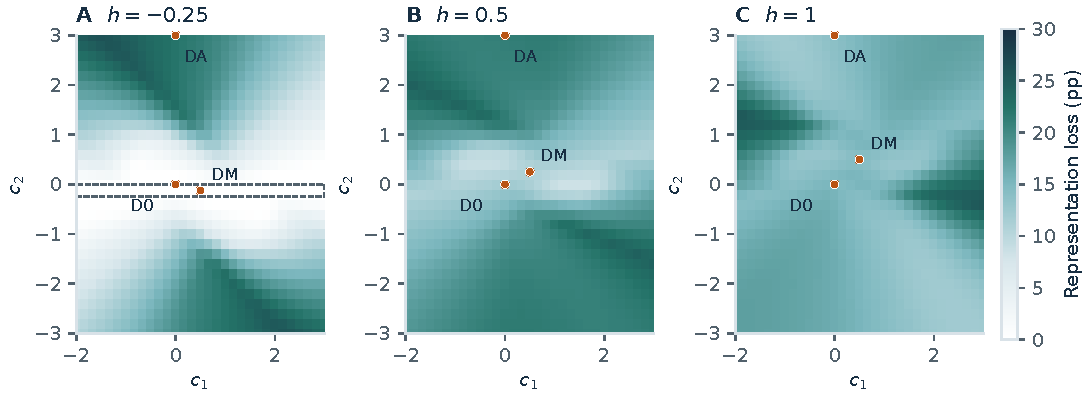
\includegraphics[width=\textwidth]{Fig2_Origin_Loss.pdf}\caption{Area-uniform representation loss across a $31\times31$ origin grid for each displacement. D0, DM and DA are the prespecified neural origins. Grid values use midpoint angular quadrature checked by refinement; marked origins also have rigorous risk enclosures.}\label{fig:originmap}\end{figure}
Table~\ref{tab:diagnostic-supp} reports the capacity, conditioning and radius-retention contrasts. Figure~\ref{fig:neural-supp} displays each seed's error alongside its population floor. Figure~\ref{fig:contrast-supp} compares the learned contrasts and deterministic population contrasts. Figure~\ref{fig:density-supp} shows that changing the sampling measure changes loss even on identical supports. All tested positive density-loss differences range from approximately 0.0813 to 0.2278 percentage points, with their propagated integration intervals excluding zero.
\begin{figure}[htbp]\centering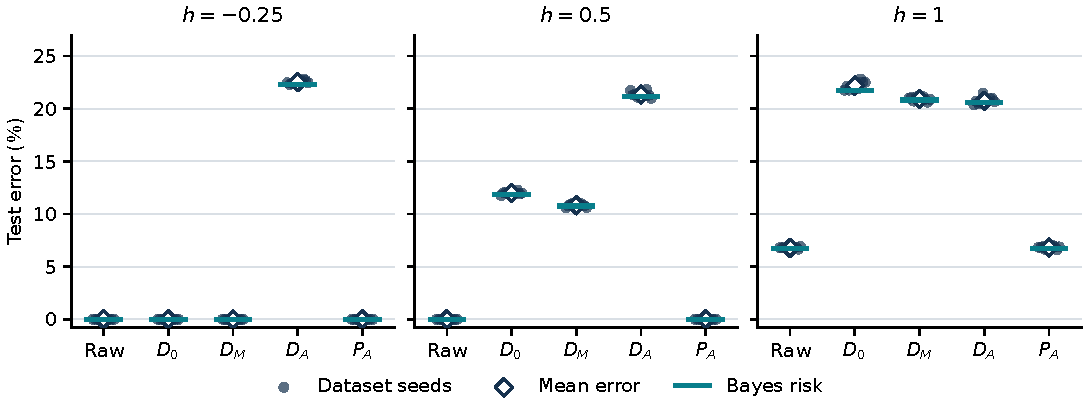
\includegraphics[width=\textwidth]{Neural_Error_and_Oracle_Floors_h.pdf}\caption{All ten seed outcomes for the 15 primary conditions. Horizontal bars are population Bayes risks; diamonds are neural means.}\label{fig:neural-supp}\end{figure}
\begin{figure}[htbp]\centering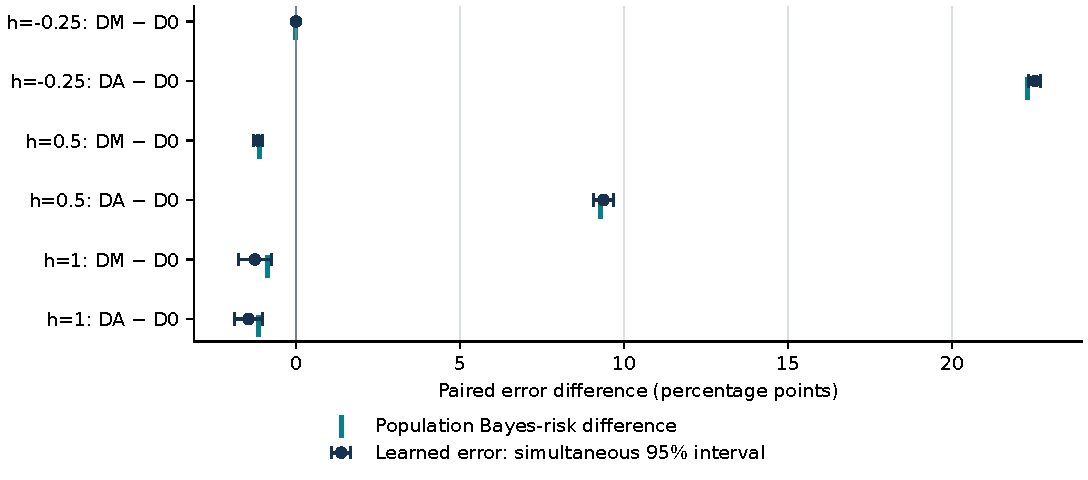
\includegraphics[width=\textwidth]{Origin_Contrast_Intervals_h.pdf}\caption{Six primary learned origin contrasts with simultaneous 95\% paired-$t$ intervals and the corresponding population Bayes-risk differences.}\label{fig:contrast-supp}\end{figure}
\begin{figure}[htbp]\centering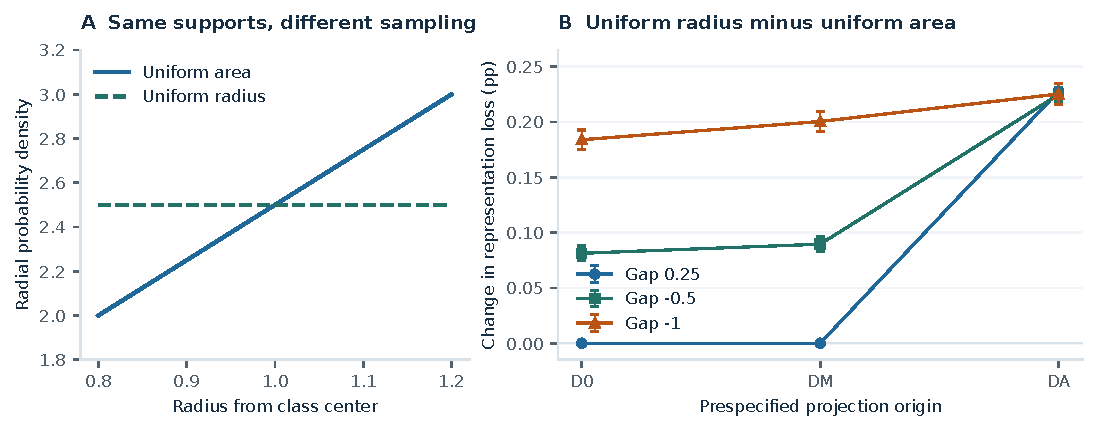
\includegraphics[width=\textwidth]{Density_Control.pdf}\caption{Sampling density and representation loss. (A) Radius distributions for uniform-area and uniform-radius sampling. (B) Change in population loss after replacing uniform area by uniform radius; error bars propagate certified integration intervals. This figure retains the archived gap notation $g=-h$.}\label{fig:density-supp}\end{figure}
\section{Independent neural experiment for the one-bit repair}
\label{supp:one-bit-experiment}

The added experiment used the same area-uniform $h=0.5$ population with fresh random streams. Its four representations were raw coordinates $R$, midpoint directions $D_M$, midpoint directions and $q=\mathbf1\{\rho>0.8\}$ ($B$), and midpoint directions and the continuous radius $\rho$ ($P_M$). All normalization origins were $(0.5,0.25)$. Population exploration and the geometric construction preceded the new protocol; the radial threshold was fixed before generating its training, validation or test observations. The original experiment's hyperparameters were reused without additional search.

Seeds 2001--2010 used NumPy \texttt{SeedSequence([941209,404,0,seed,split])}, with split identifiers 0, 1 and 2 for training, validation and test. Initializations used \texttt{SeedSequence([941209,404,9,seed])}. These streams differ from the original study namespace 641203. Each seed supplied balanced sets of 2,000 training, 2,000 validation and 50,000 test observations. The four representations shared observations and nested initial weights. The bit and radius conditions each have three inputs and 321 trainable parameters, compared with two inputs and 257 parameters for raw and direction conditions. Every network has 64 tanh hidden units and a linear output.

Full-batch Adam, MSE labels $-1/+1$, the two learning rates, conditioning, 4,000-update budget and validation selection order were unchanged. The 80 candidates executed 320,000 updates and 640 million training-example exposures, taking 313.90 seconds on two CPU workers. All 40 selections were frozen before test generation. The test evaluator checked source identities and the release record, generated the ten fresh test sets, and evaluated each selected model once. The frozen explicit decoder was then evaluated on the same observations.

\begin{table}[ht]
\centering\small
\caption{Fresh one-bit experiment: misclassified observations out of 50,000 per seed and representation. The explicit decoder made zero errors for every seed.}
\label{supp:tab:bit-seeds}
\begin{tabular}{rrrrr}
\toprule
Seed & $R$ & $D_M$ & $B$ & $P_M$\\
\midrule
2001&0&5388&0&0\\
2002&0&5514&0&0\\
2003&0&5528&3&0\\
2004&0&5461&0&0\\
2005&0&5340&0&0\\
2006&0&5457&0&0\\
2007&0&5392&0&0\\
2008&0&5405&0&0\\
2009&0&5444&0&0\\
2010&0&5433&0&0\\
\midrule
Total&0&54362&3&0\\
\bottomrule
\end{tabular}
\end{table}

The two prespecified primary contrasts were $B-D_M$ and $B-P_M$. Their simultaneous 95\% intervals use $t_9(1-0.05/4)$; the independent dataset/initialization seed is the analysis unit. Whole-seed bootstrap sensitivity used 10,000 resamples from \texttt{SeedSequence([941209,505,7001])}. The pointwise percentile intervals were $[-10.9388,-10.8056]$~pp for $B-D_M$ and $[0,0.0018]$~pp for $B-P_M$. The descriptive $B-R$ difference was $0.0006$~pp with pointwise paired-$t$ interval $[-0.0008,0.0020]$; $P_M-R$ was zero for every seed. The full package contains all 80 learning histories, candidate minima, 40 selected models, predictions, seed differences and bootstrap indices.

\section{Reproduction and provenance}
The archive contains \texttt{research/neural}, \texttt{research/oracles}, \texttt{research/literature}, and the analytical proofs. The neural folder preserves generated observations, all candidate training histories and optimizer checkpoints, selected weights, test scores, analysis tables, frozen manifests, independent audit records and SHA-256 checksums. The oracle folder contains exact radial integration, finite sign tests, Arb certificates, origin grids and structural controls. The literature folder contains bibliographic metadata and original audit notes. Source articles are identified through their publication links.

Run the documented analysis command against the saved test results to regenerate tables. The independent completion-audit script reconstructs predictions and statistics from saved weights and observations. The release and completion audits verify protocol, data, model and output hashes; the training runner resumes saved optimizer checkpoints. The README states environment versions, clean rerun options and build order for the article and supplement. Reproducing training can vary in wall time across hardware; the completed audit establishes exact prediction and analysis reconstruction in the recorded environment.
\bibliographystyle{unsrtnat}
\bibliography{references}
\end{document}
